\documentclass{article}

% Set the margins of the page.
\usepackage[a4paper, total={6.5in, 9in}]{geometry}

% A bunch of math packages.
\usepackage{amssymb}
\usepackage{amsmath}
\usepackage{amsthm}
\usepackage{amsfonts}
\usepackage{mathtools}
\usepackage{float}

\usepackage{changepage}
\usepackage{graphicx} 		% Insert images
\usepackage{color}				% COLORS!
\usepackage[shortlabels]{enumitem}			% More enumerate types such as \alph*
\usepackage{listings}			% Used for code-blocks in latex.
\usepackage{hyperref}
% Create links when using ref and table of contents.
\hypersetup{colorlinks=true, linkcolor=black}

% Replace the indents for paragraphs with empty lines.
\usepackage[parfill]{parskip}

\usepackage[myheadings]{fancyhdr}
\usepackage{titleref}
\makeatletter
\newcommand*{\currentname}{\TR@currentTitle}
\makeatother

% Number equations with reference to sub sections.
\numberwithin{equation}{subsection}

\definecolor{lightgray}{RGB}{200, 200, 200}

% Set some style rules for code-blocks
\lstset{
	literate={<-}{$\leftarrow$}{2} {\\infty}{$\infty$}{1},
	backgroundcolor=\color{lightgray}
,
	framexleftmargin=2pt,
	framexrightmargin=2pt,
	framextopmargin=2pt,
	framexbottommargin=2pt,
	frame=single,
	basicstyle=\fontsize{10pt}{15pt}\selectfont,
	stepnumber=1,
	tabsize=4,
}


%increases table padding
\def\arraystretch{1.5}



\title{\textbf{CSCI-4116\\Assignment 1}}
\author{Anas Alhadi\\B00895875}


\begin{document}

	\maketitle
	\tableofcontents


	\newpage
	\section{Exercise 1}
	\subsection{Q1 and 2}
	\begin{figure}[H]
		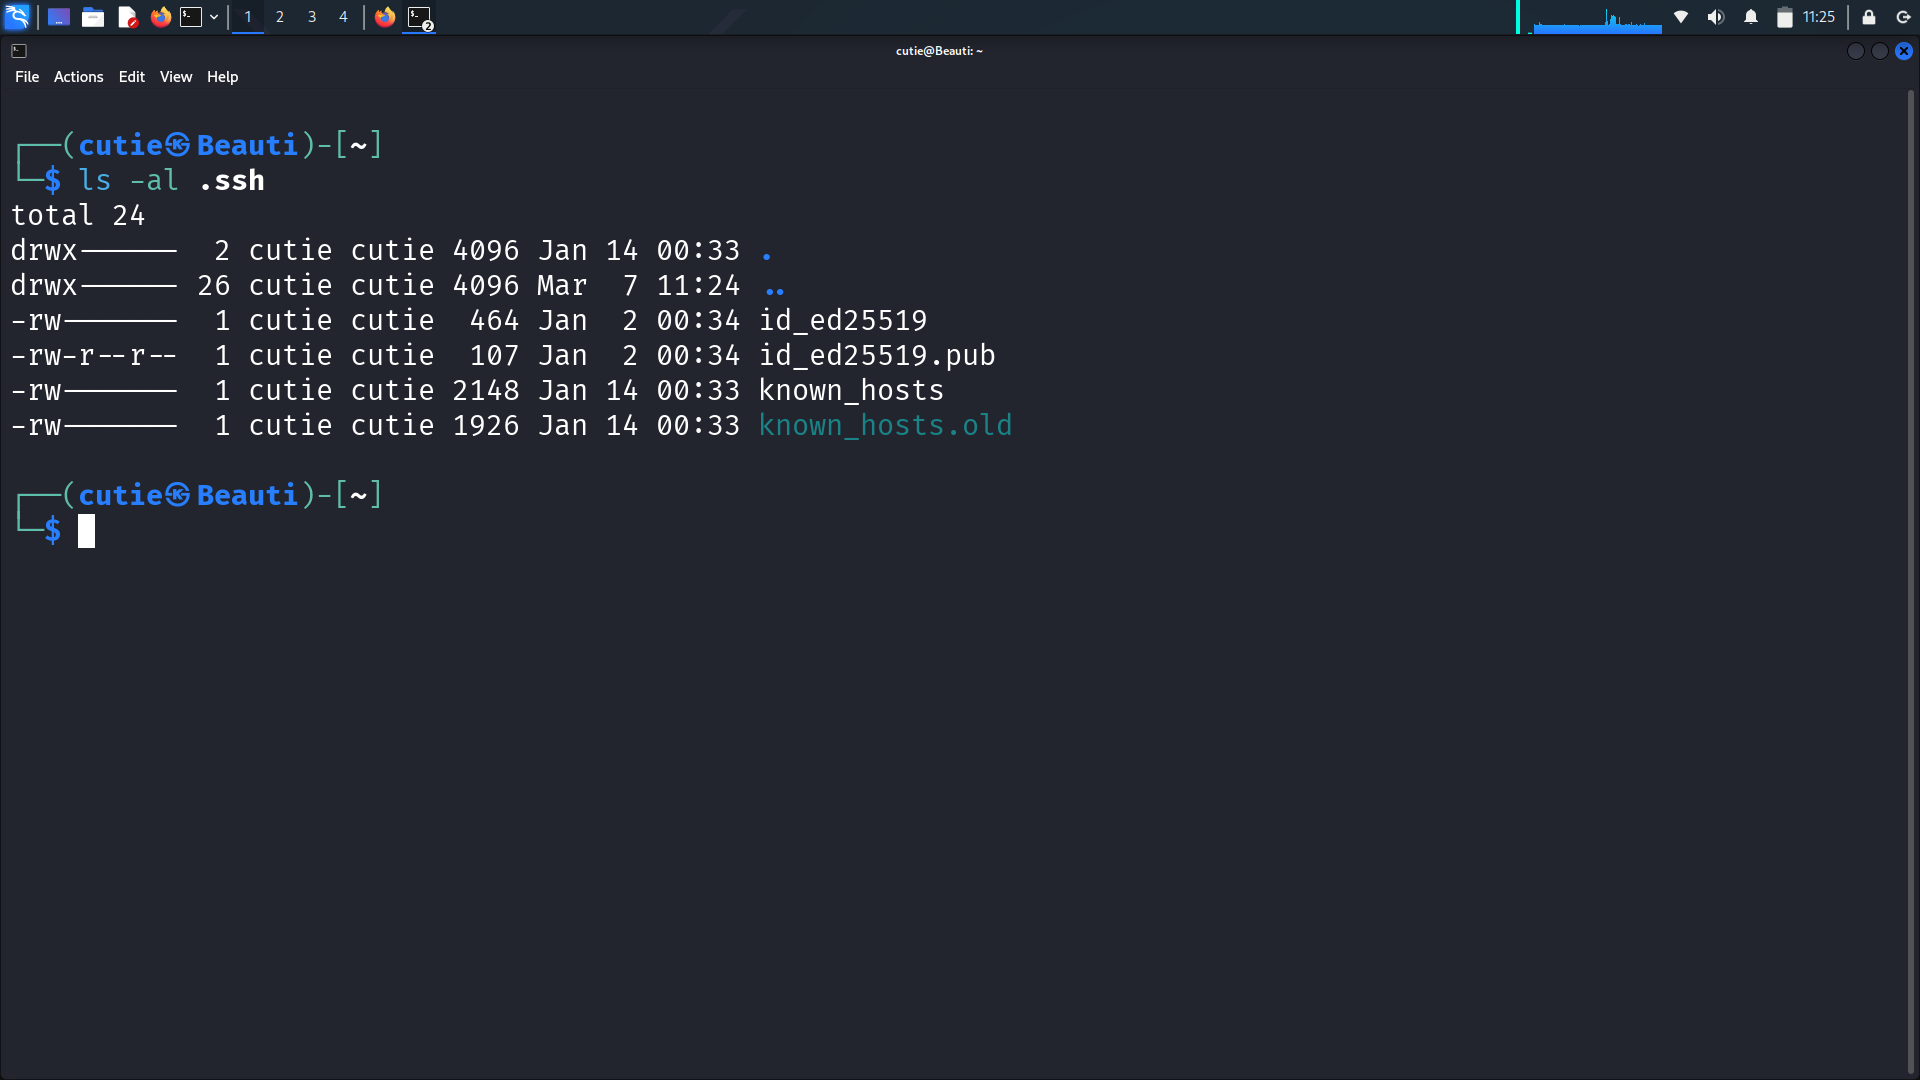
\includegraphics[width=430pt]{pics/q1/1.png}
	\end{figure}

	\vspace{25pt}

	\subsection{Q3}
	\begin{figure}[H]
		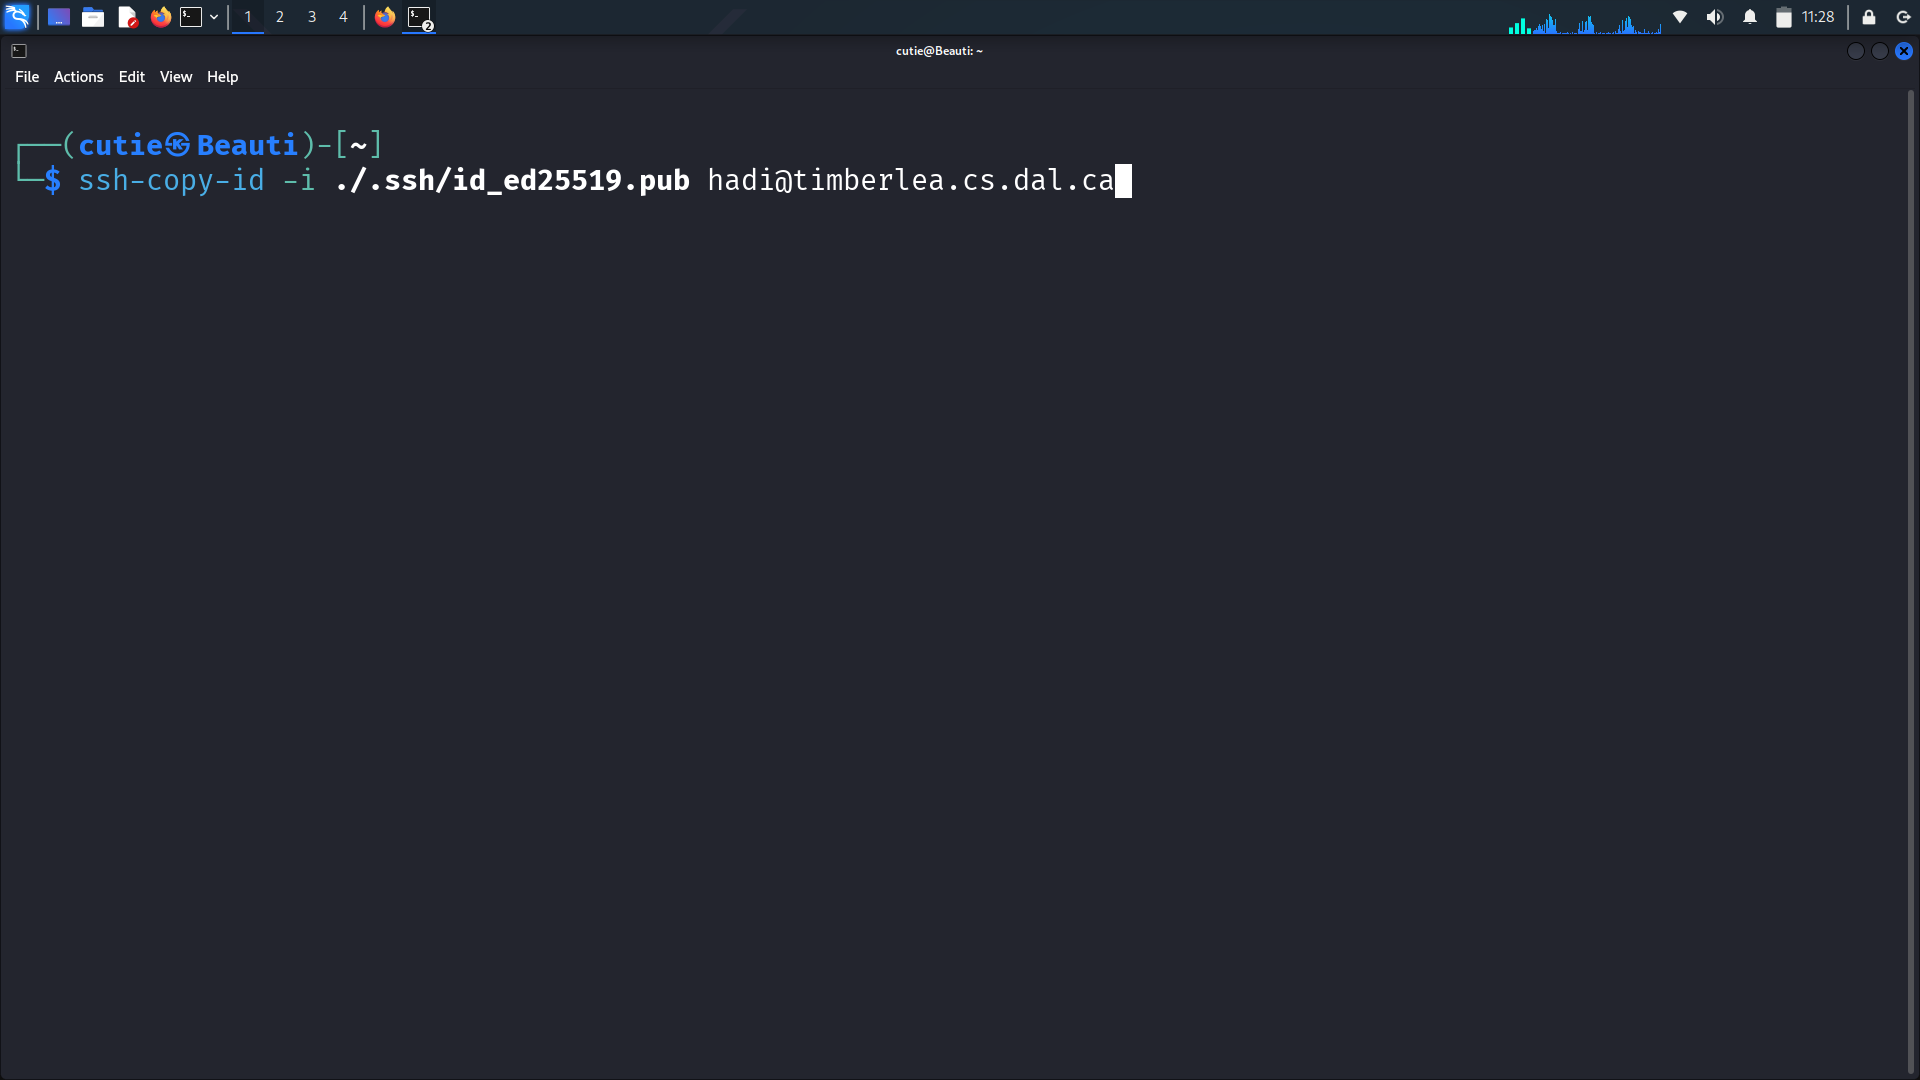
\includegraphics[width=430pt]{pics/q1/2.png}
	\end{figure}


	\vspace{25pt}

	\subsection{Q4}
	\begin{figure}[H]
		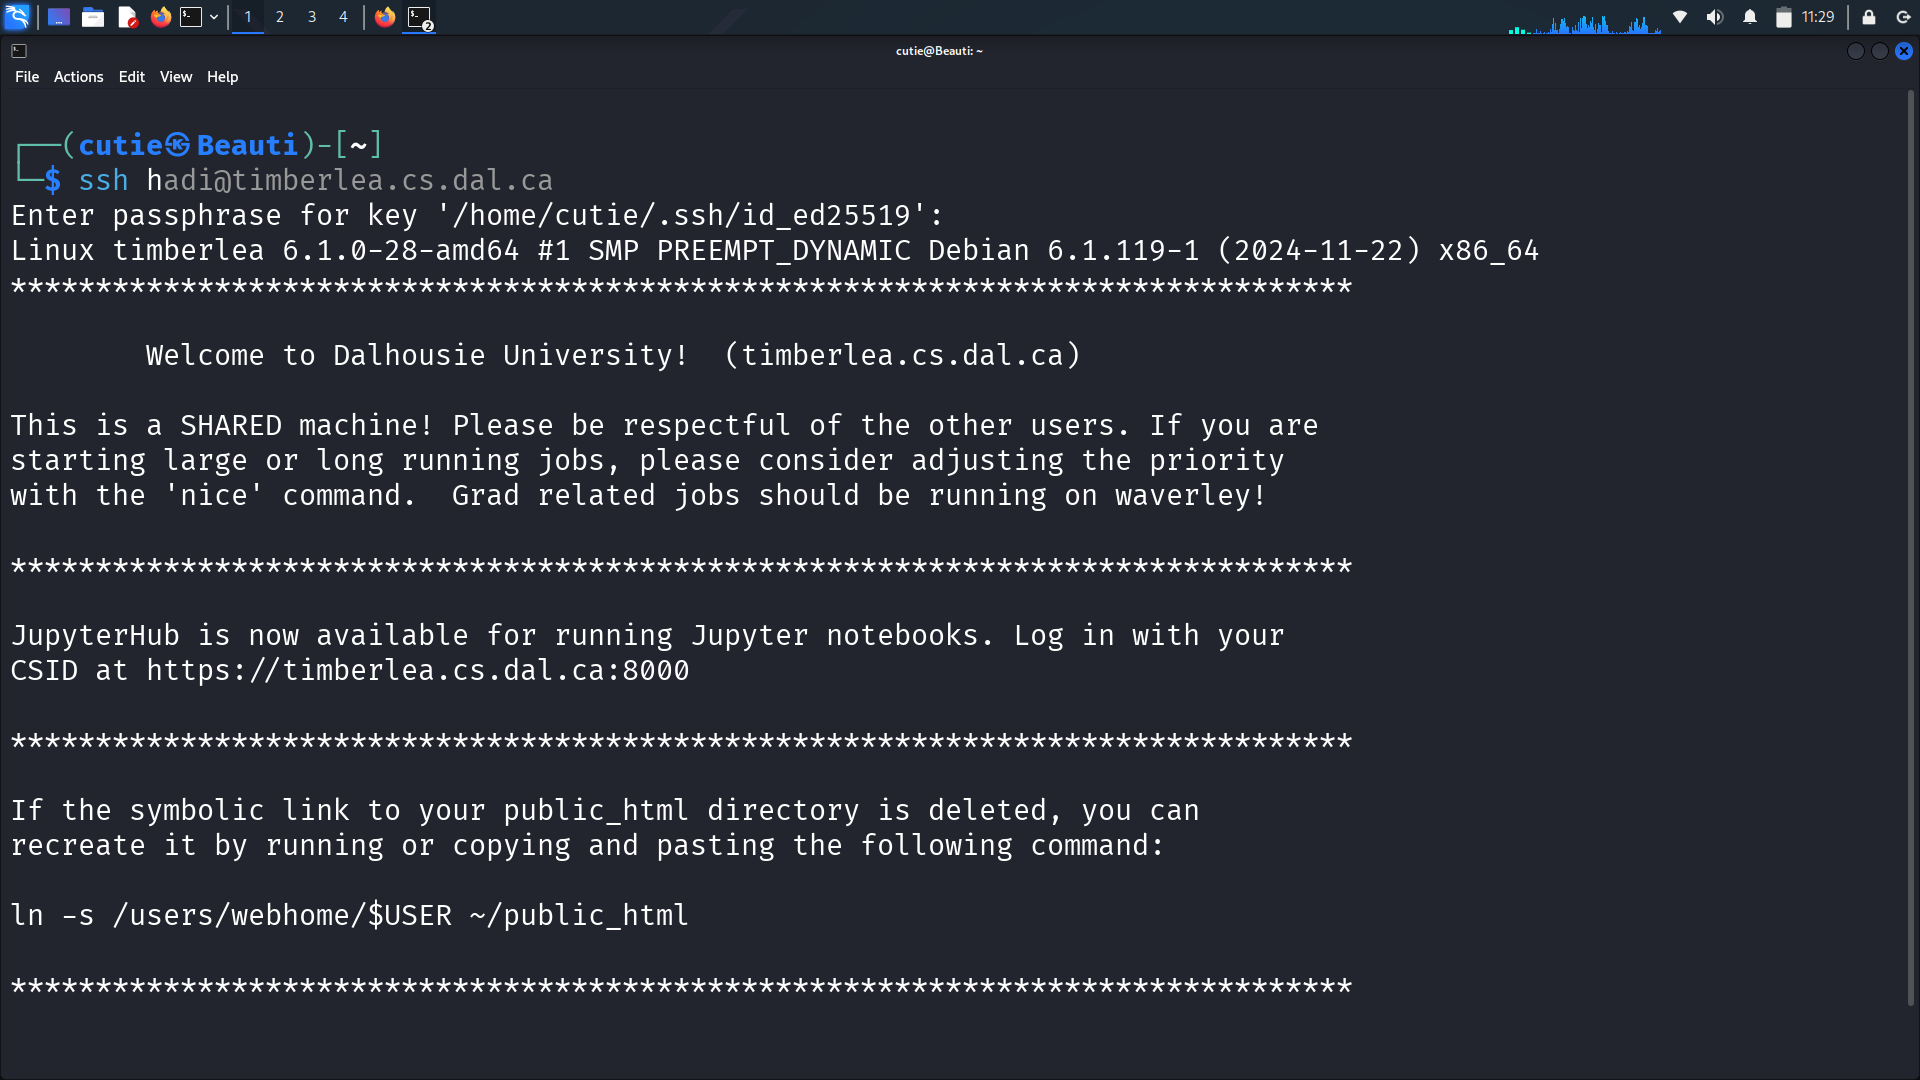
\includegraphics[width=430pt]{pics/q1/3.png}
	\end{figure}

	
	\vspace{25pt}
	\subsection{Q5}
	\begin{enumerate}
		\item \textbf{Benefits:}
			\begin{itemize}
				\item More resilient to brute force attacksas the keysize is much larger than 
					usual passwords
				\item More resilient to social engineering attacks since it is much harder to
					extract information about the key from the user (the only way to do so is to have the user share
					their private key which is easier to avoid as opposed to sharing general information that might
					hint to possible user created passwords)
				\item Does not require the user to memorize passwords
			\end{itemize}		

			\item \textbf{Drawback:}
				\begin{itemize}
					\item Requires more complex/involved setup as opposed to passwords.
					\item Requires key managment, since losing the key means that the user
						will not be able to login anymore (so a backup/key recovery mechanisim must be used in conjunction)
				\end{itemize}
		
	\end{enumerate}
	\newpage
	\section{Question 2}

	\subsection{Part 1}
	\begin{figure}[H]
		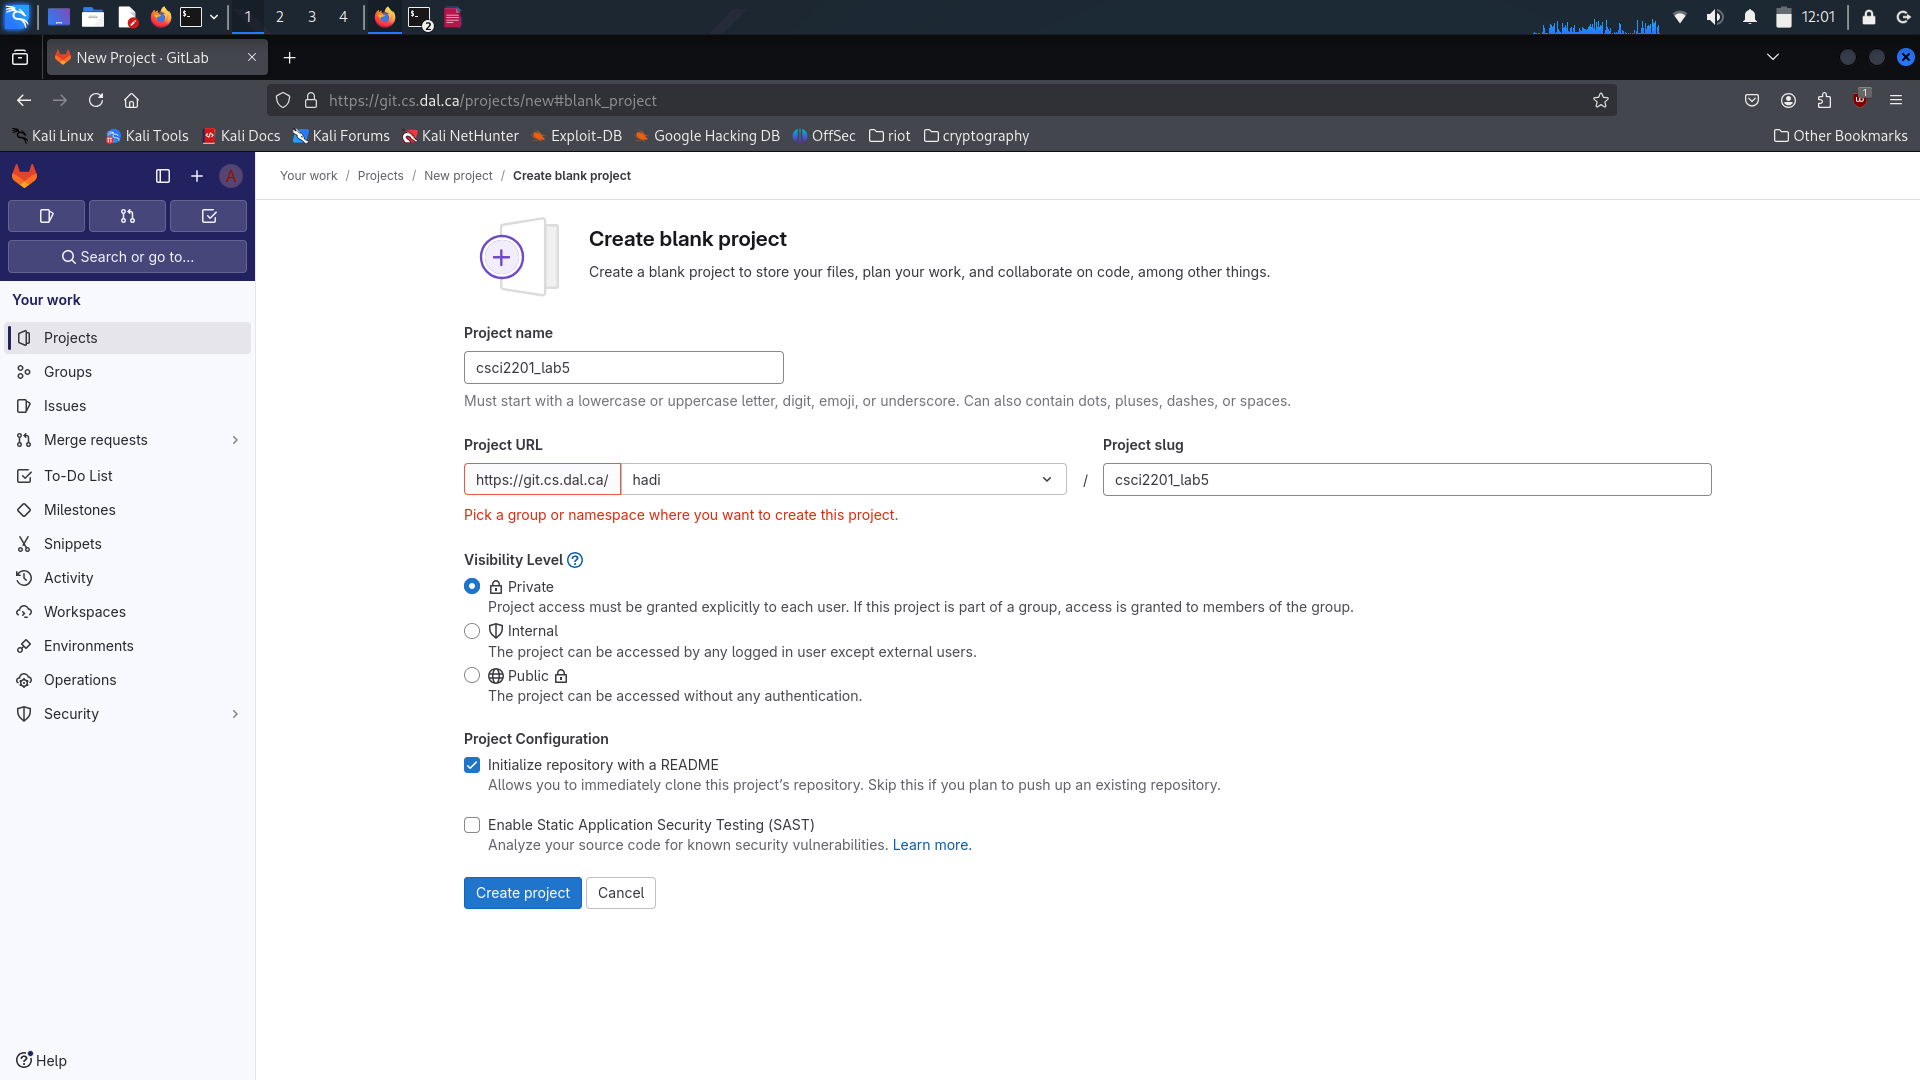
\includegraphics[width=430pt]{pics/Screenshot_2025-03-07_12_01_55.png}
	\end{figure}
	\begin{figure}[H]
		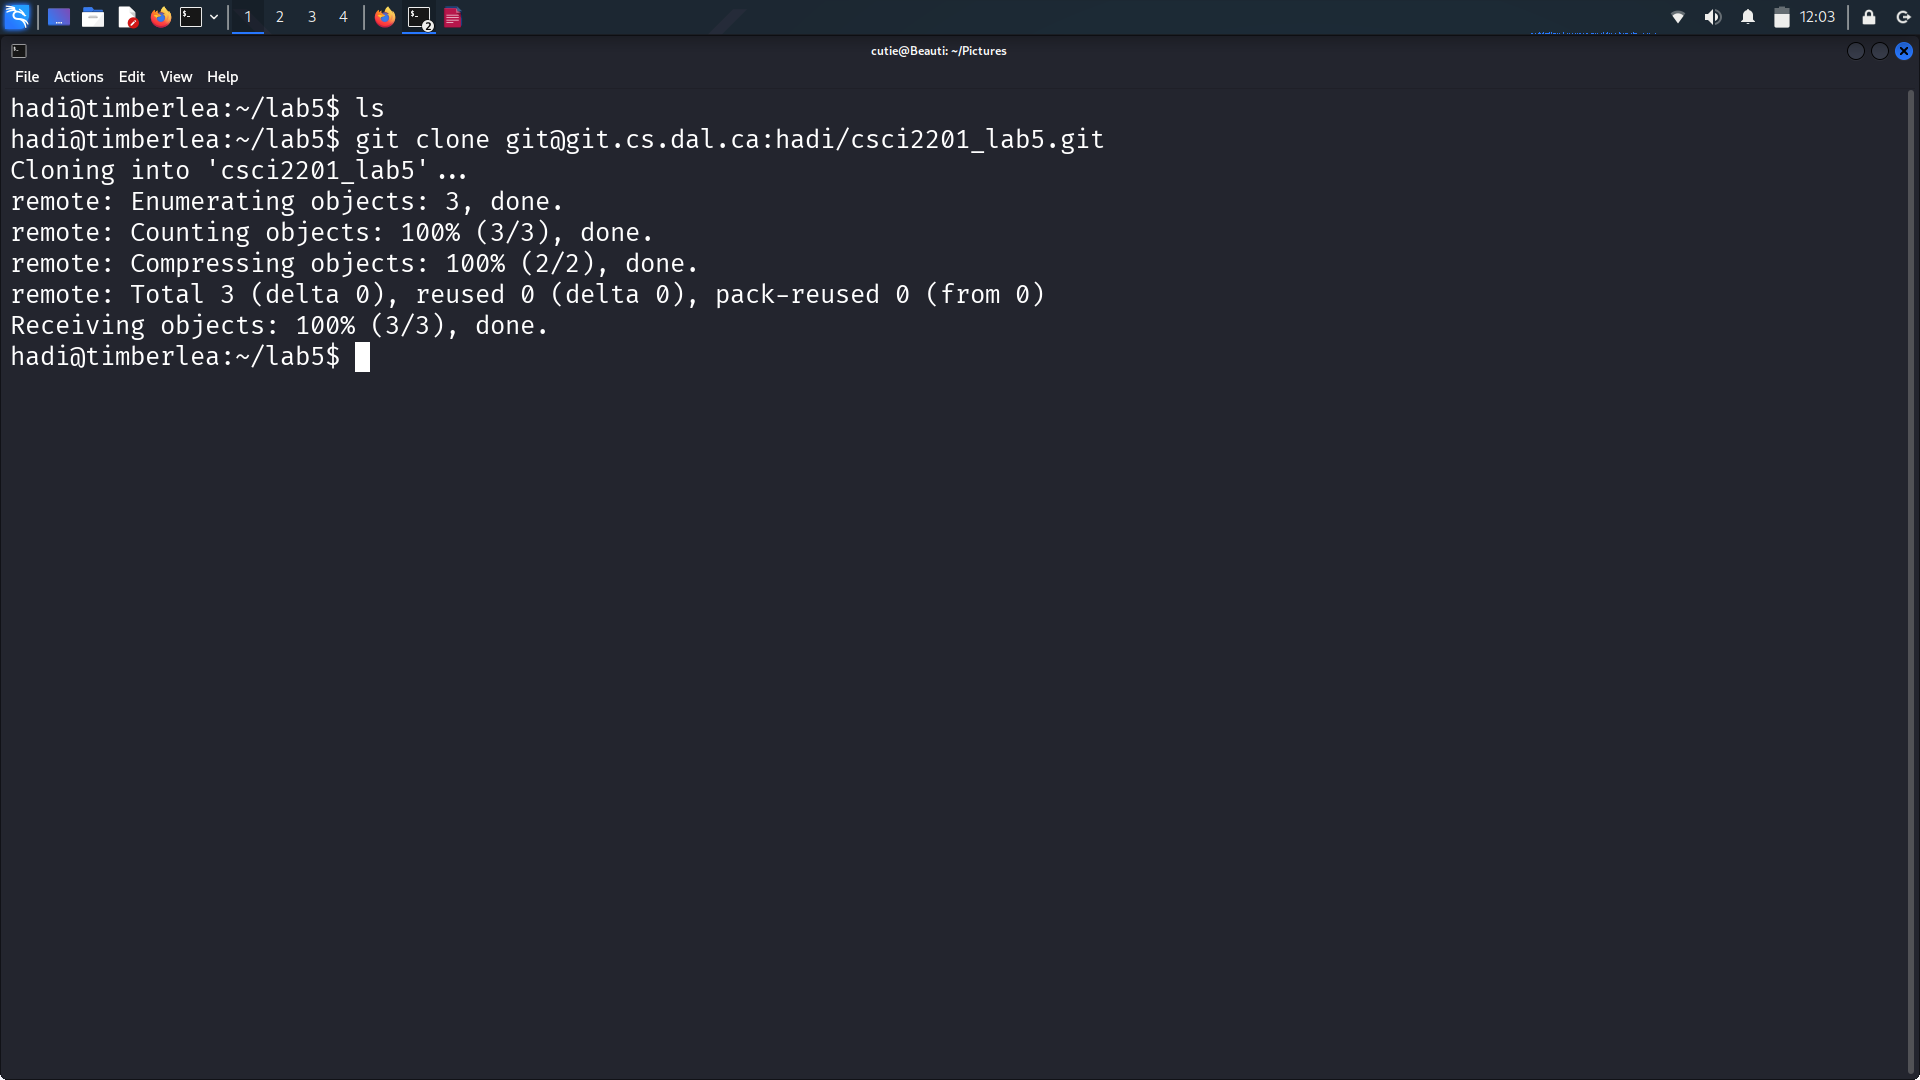
\includegraphics[width=430pt]{pics/Screenshot_2025-03-07_12_03_18.png}
	\end{figure}


	\newpage
	\subsection{Part 2}
	\begin{figure}[H]
		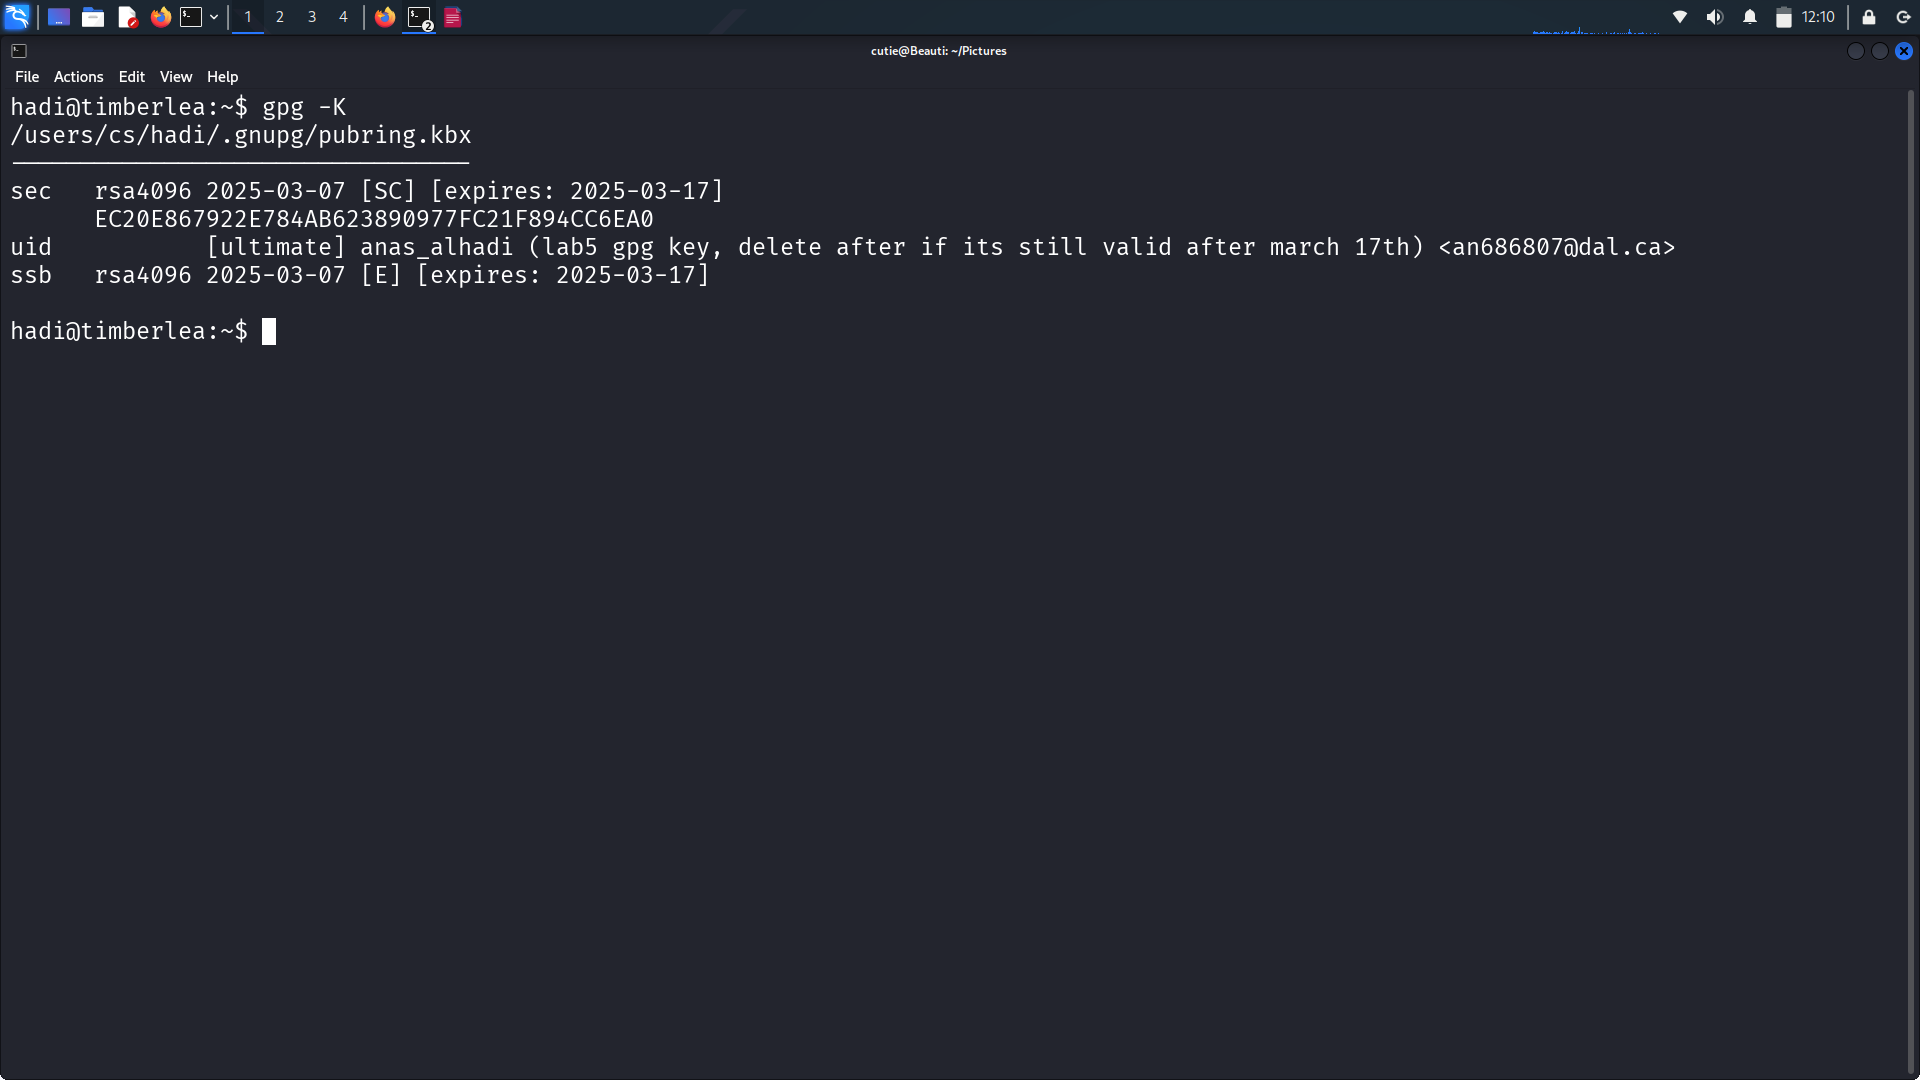
\includegraphics[width=430pt]{pics/Screenshot_2025-03-07_12_10_50.png}
	\end{figure}
	\begin{figure}[H]
		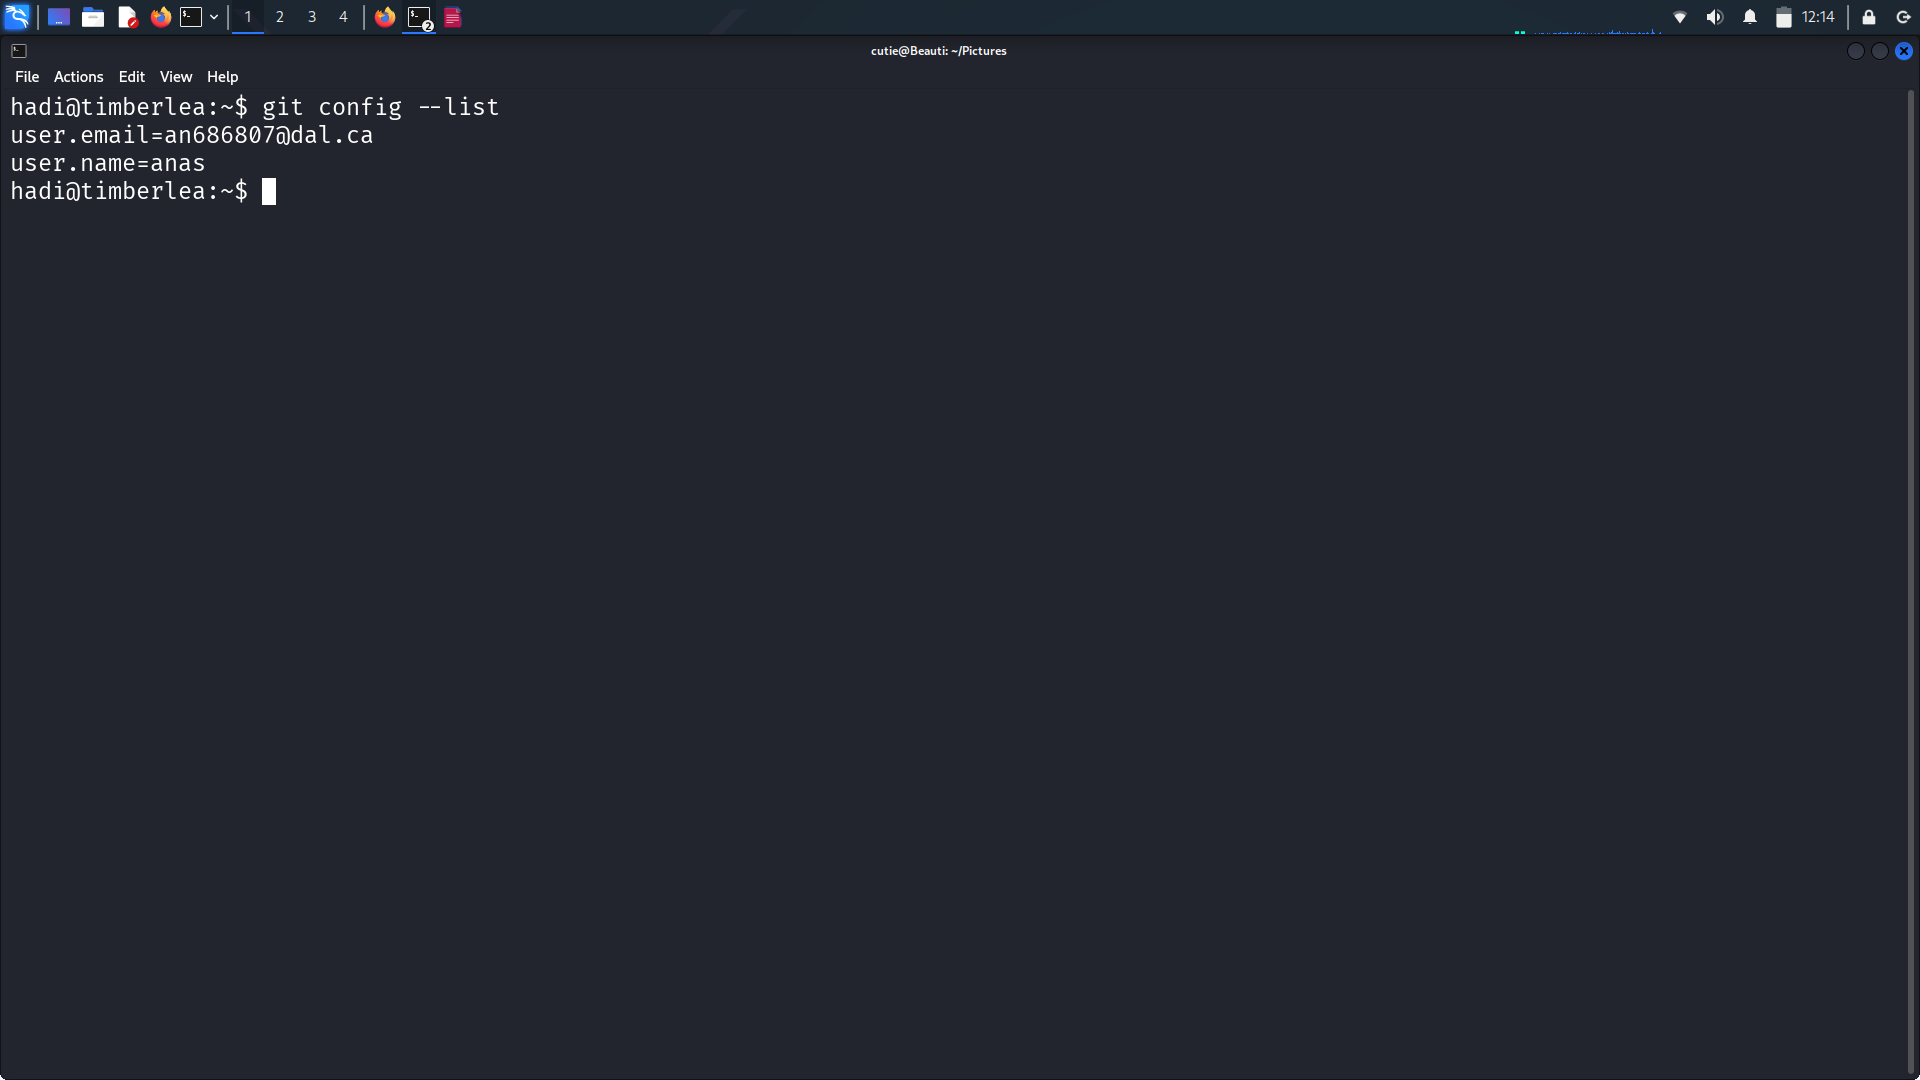
\includegraphics[width=430pt]{pics/Screenshot_2025-03-07_12_14_42.png}
	\end{figure}

	\newpage
	\subsection{Part 3}
	\begin{figure}[H]
		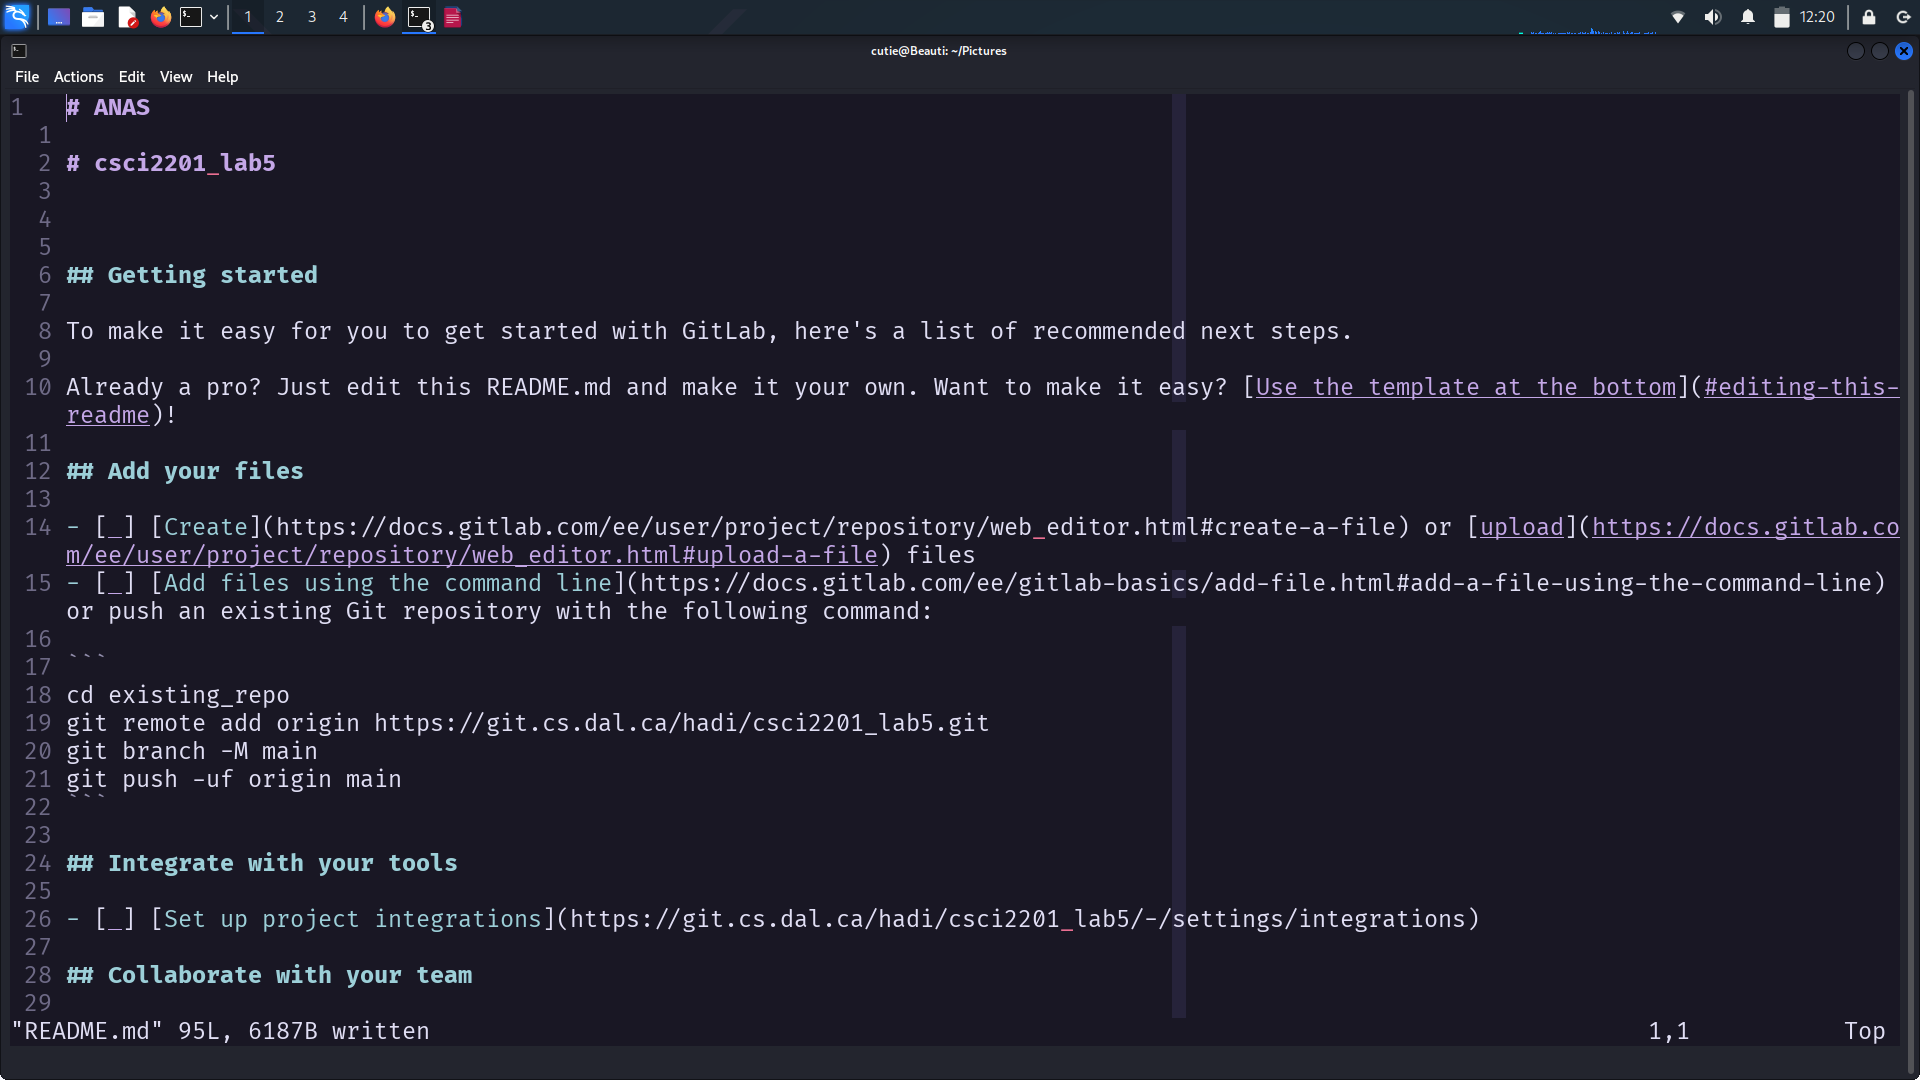
\includegraphics[width=430pt]{pics/Screenshot_2025-03-07_12_20_15.png}
	\end{figure}
	\begin{figure}[H]
		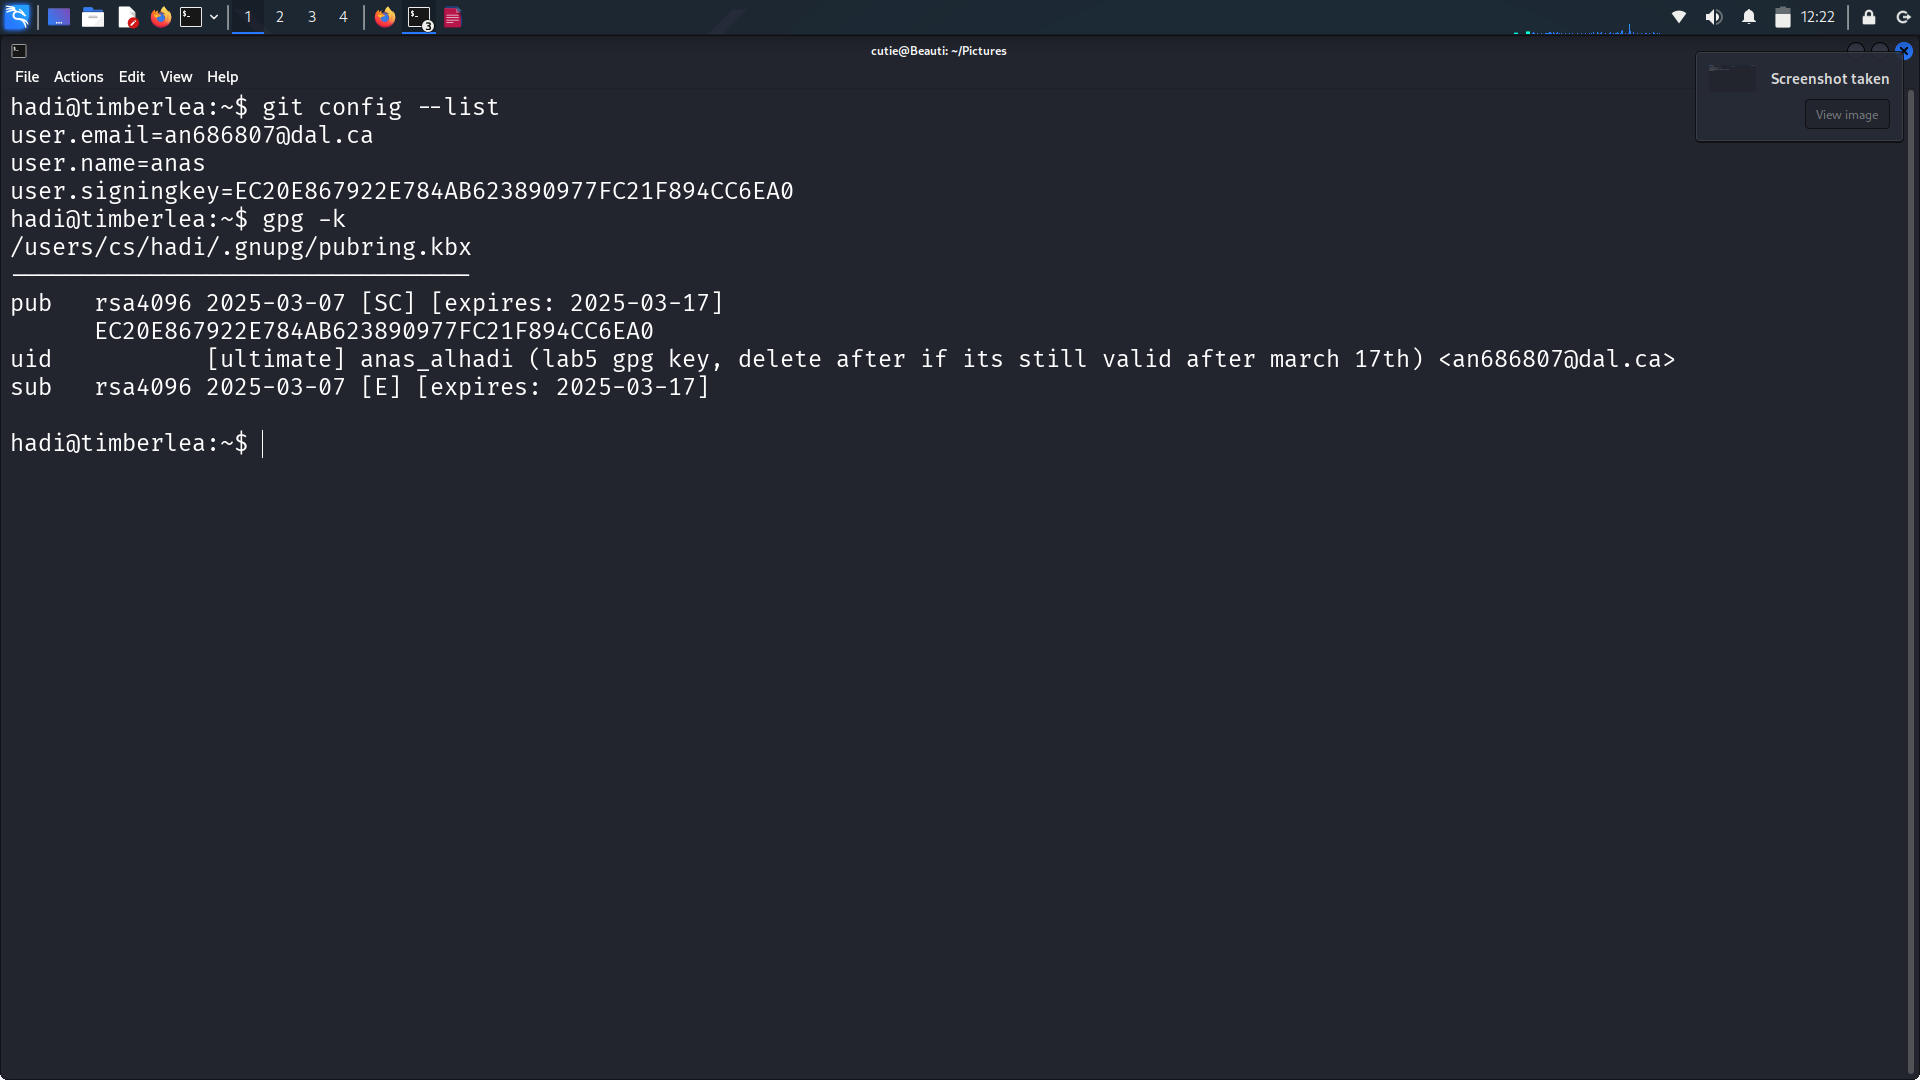
\includegraphics[width=430pt]{pics/Screenshot_2025-03-07_12_22_40.png}
	\end{figure}
	\begin{figure}[H]
		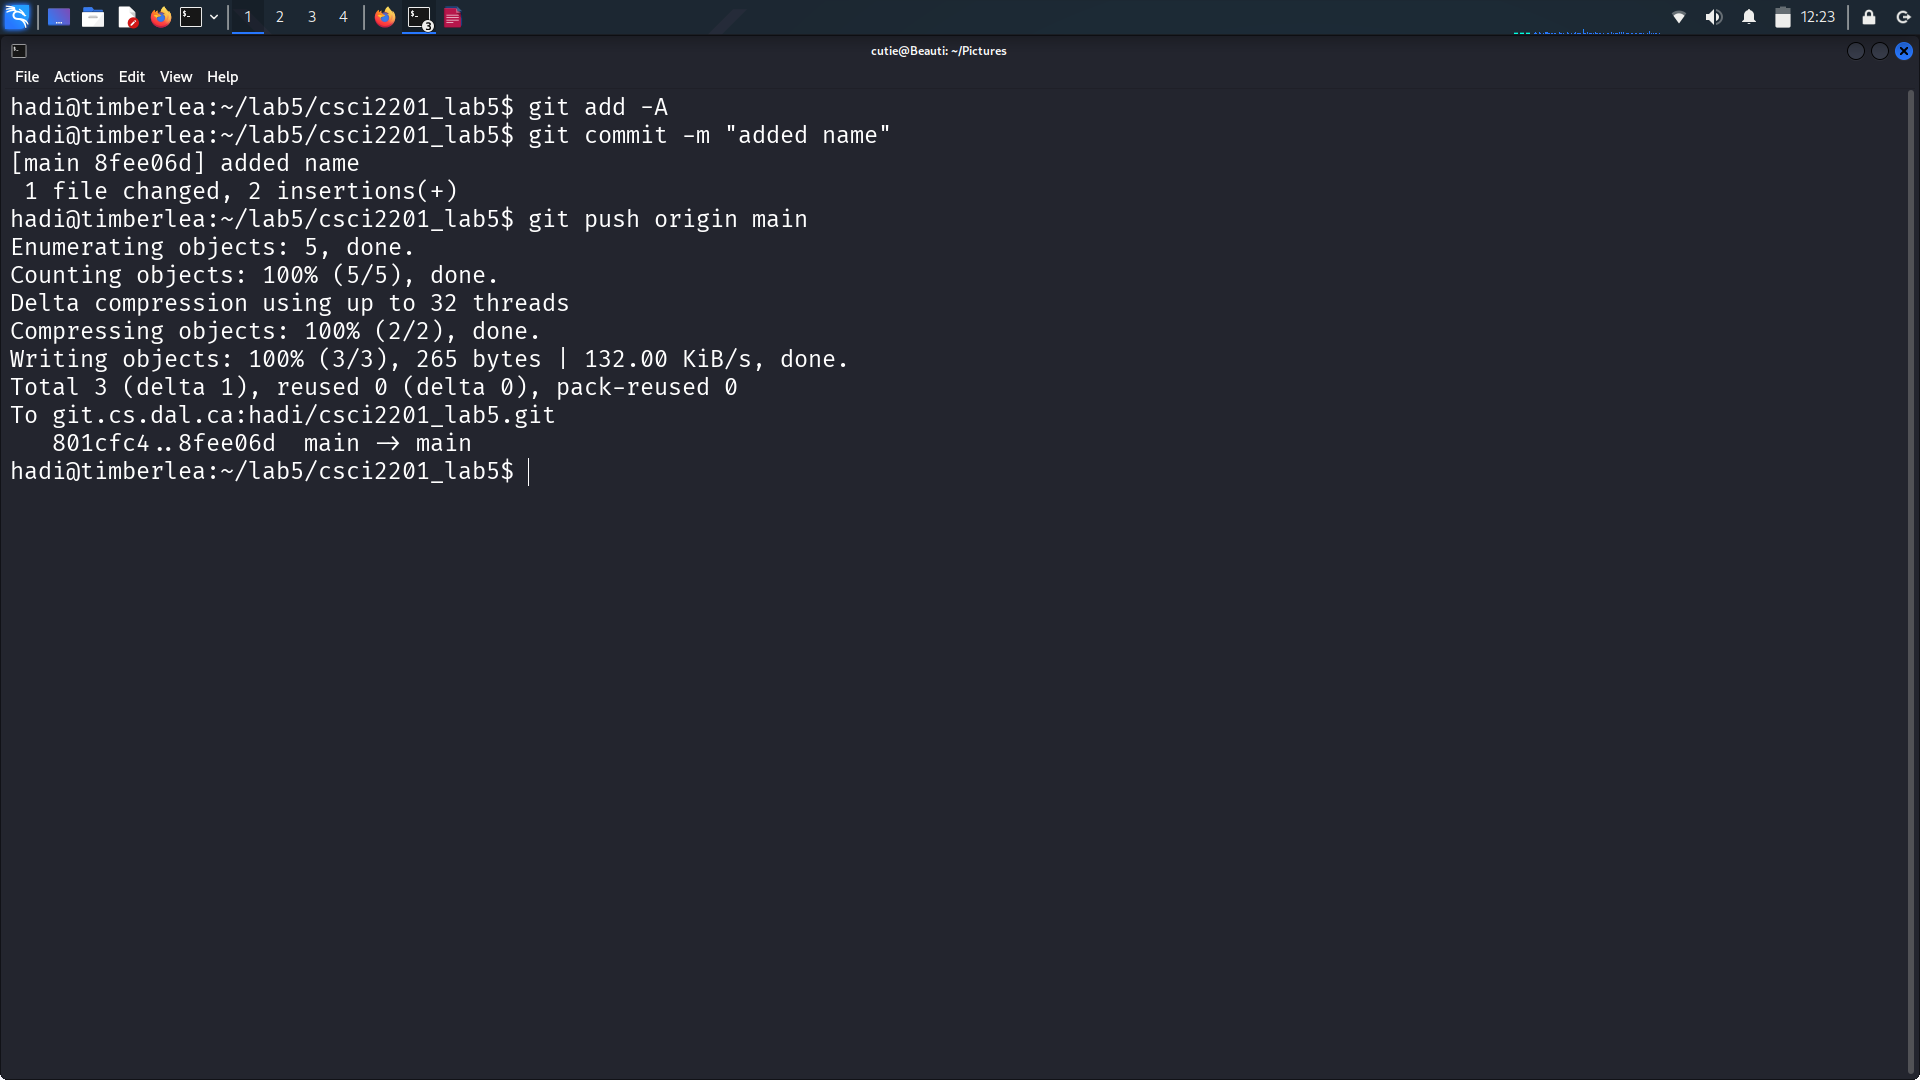
\includegraphics[width=430pt]{pics/Screenshot_2025-03-07_12_23_50.png}
	\end{figure}


	\newpage
	\subsection{Part 4}
		\begin{figure}[H]
		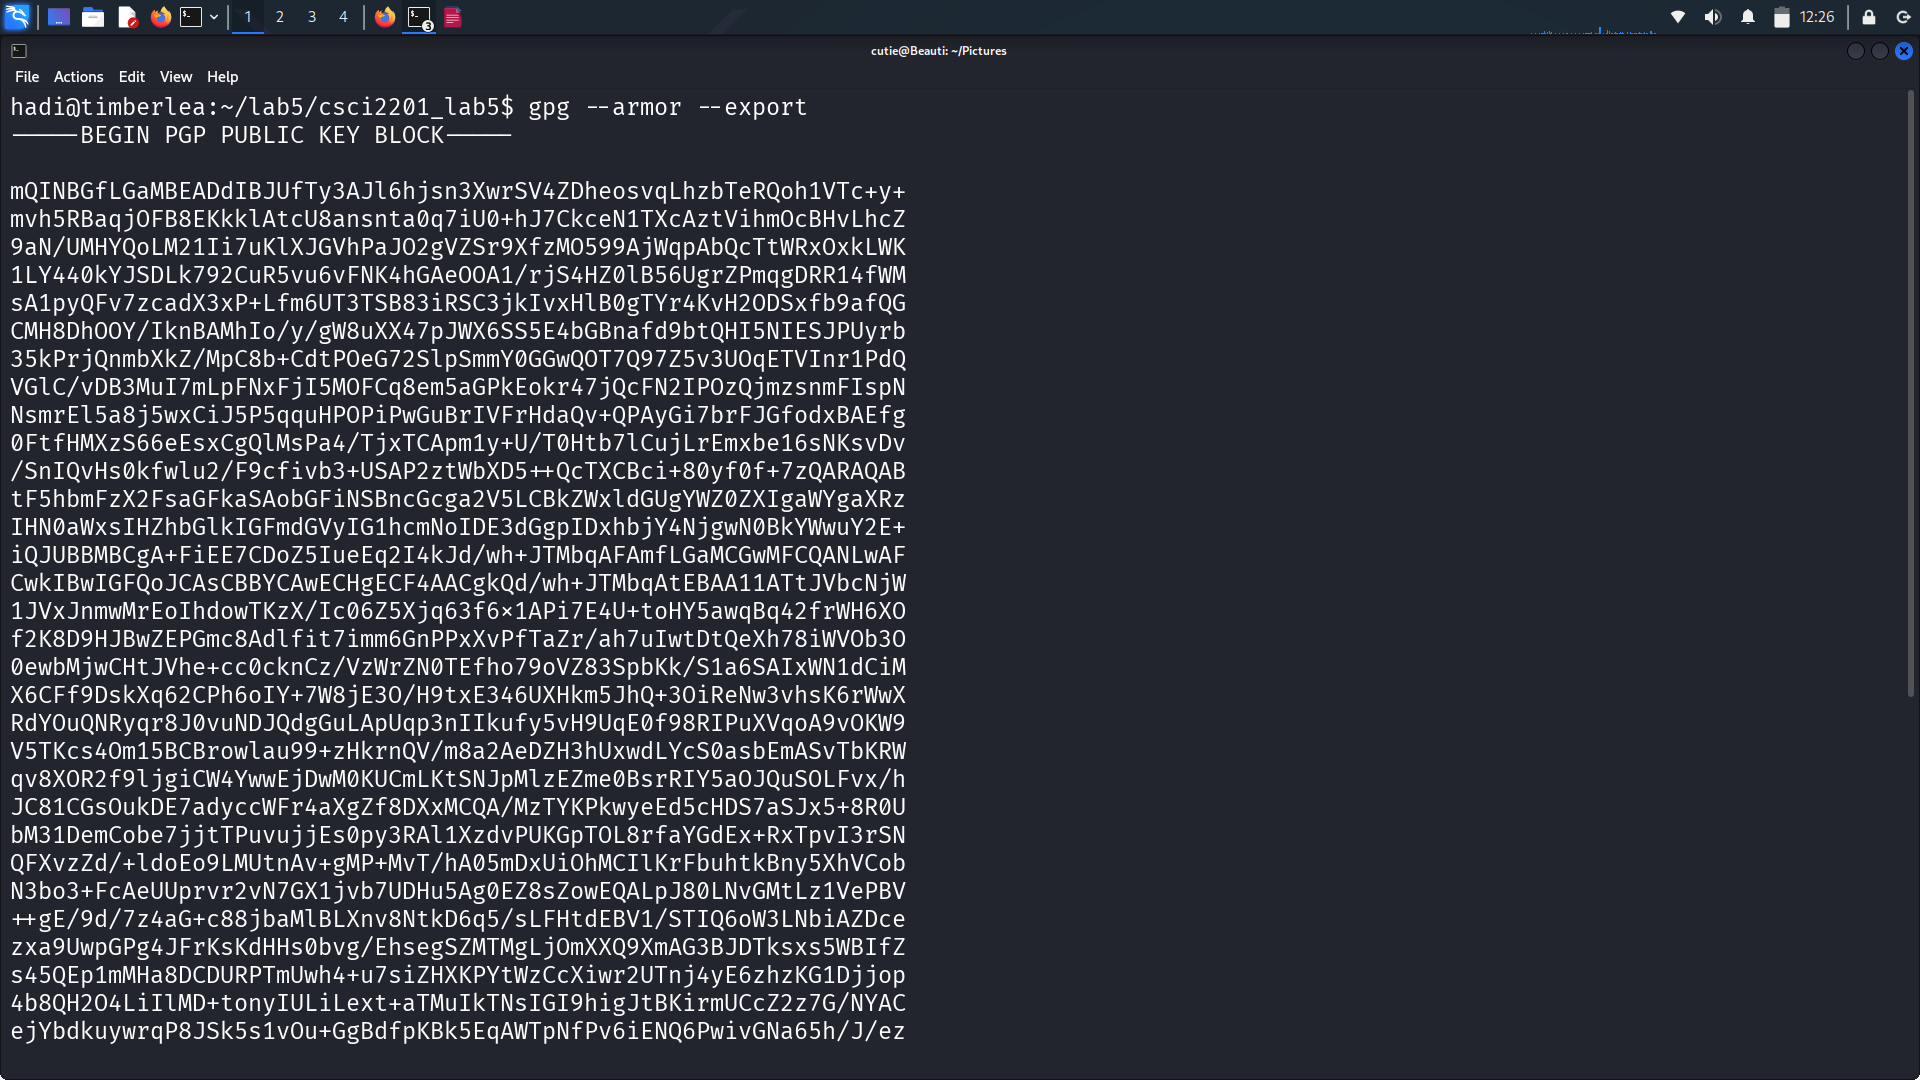
\includegraphics[width=430pt]{pics/Screenshot_2025-03-07_12_26_47.png}
	\end{figure}
	\begin{figure}[H]
		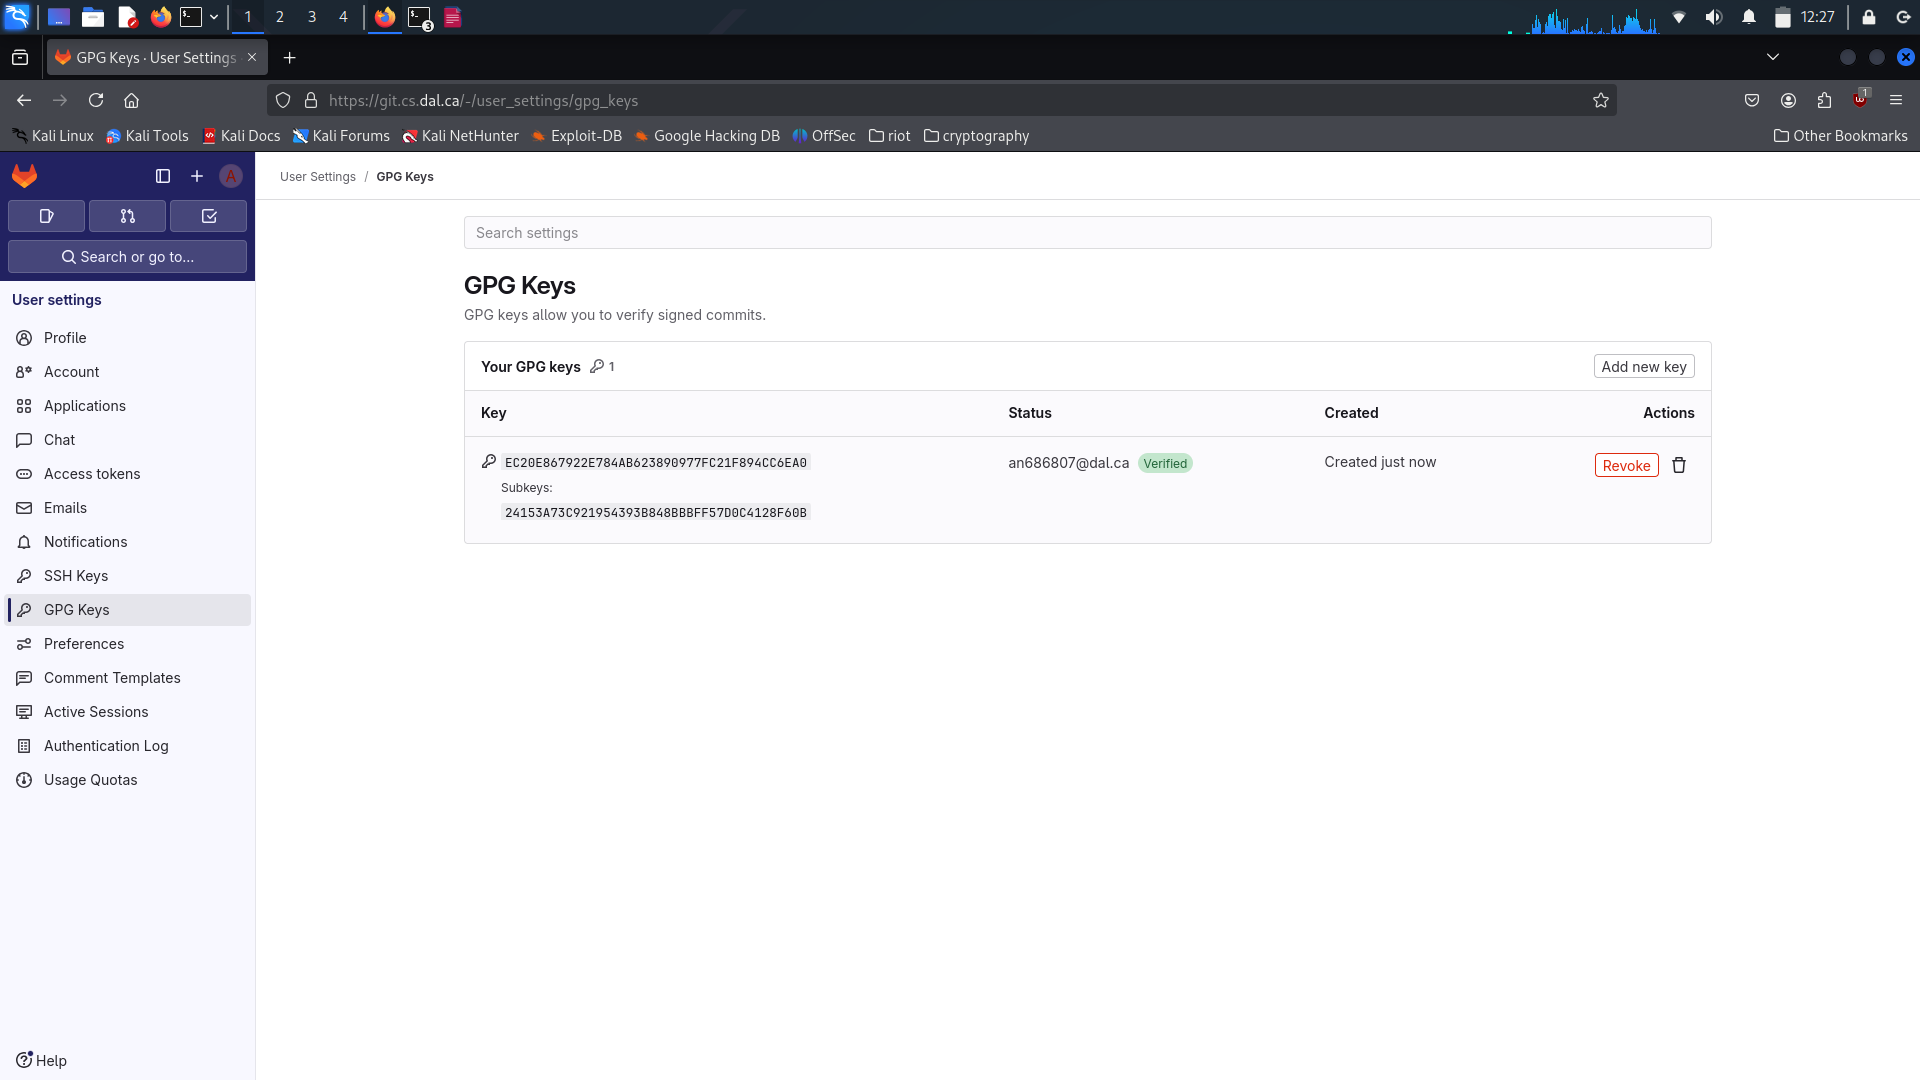
\includegraphics[width=430pt]{pics/Screenshot_2025-03-07_12_27_37.png}
	\end{figure}

	\newpage
	\subsection{Part 5}
	\begin{figure}[H]
		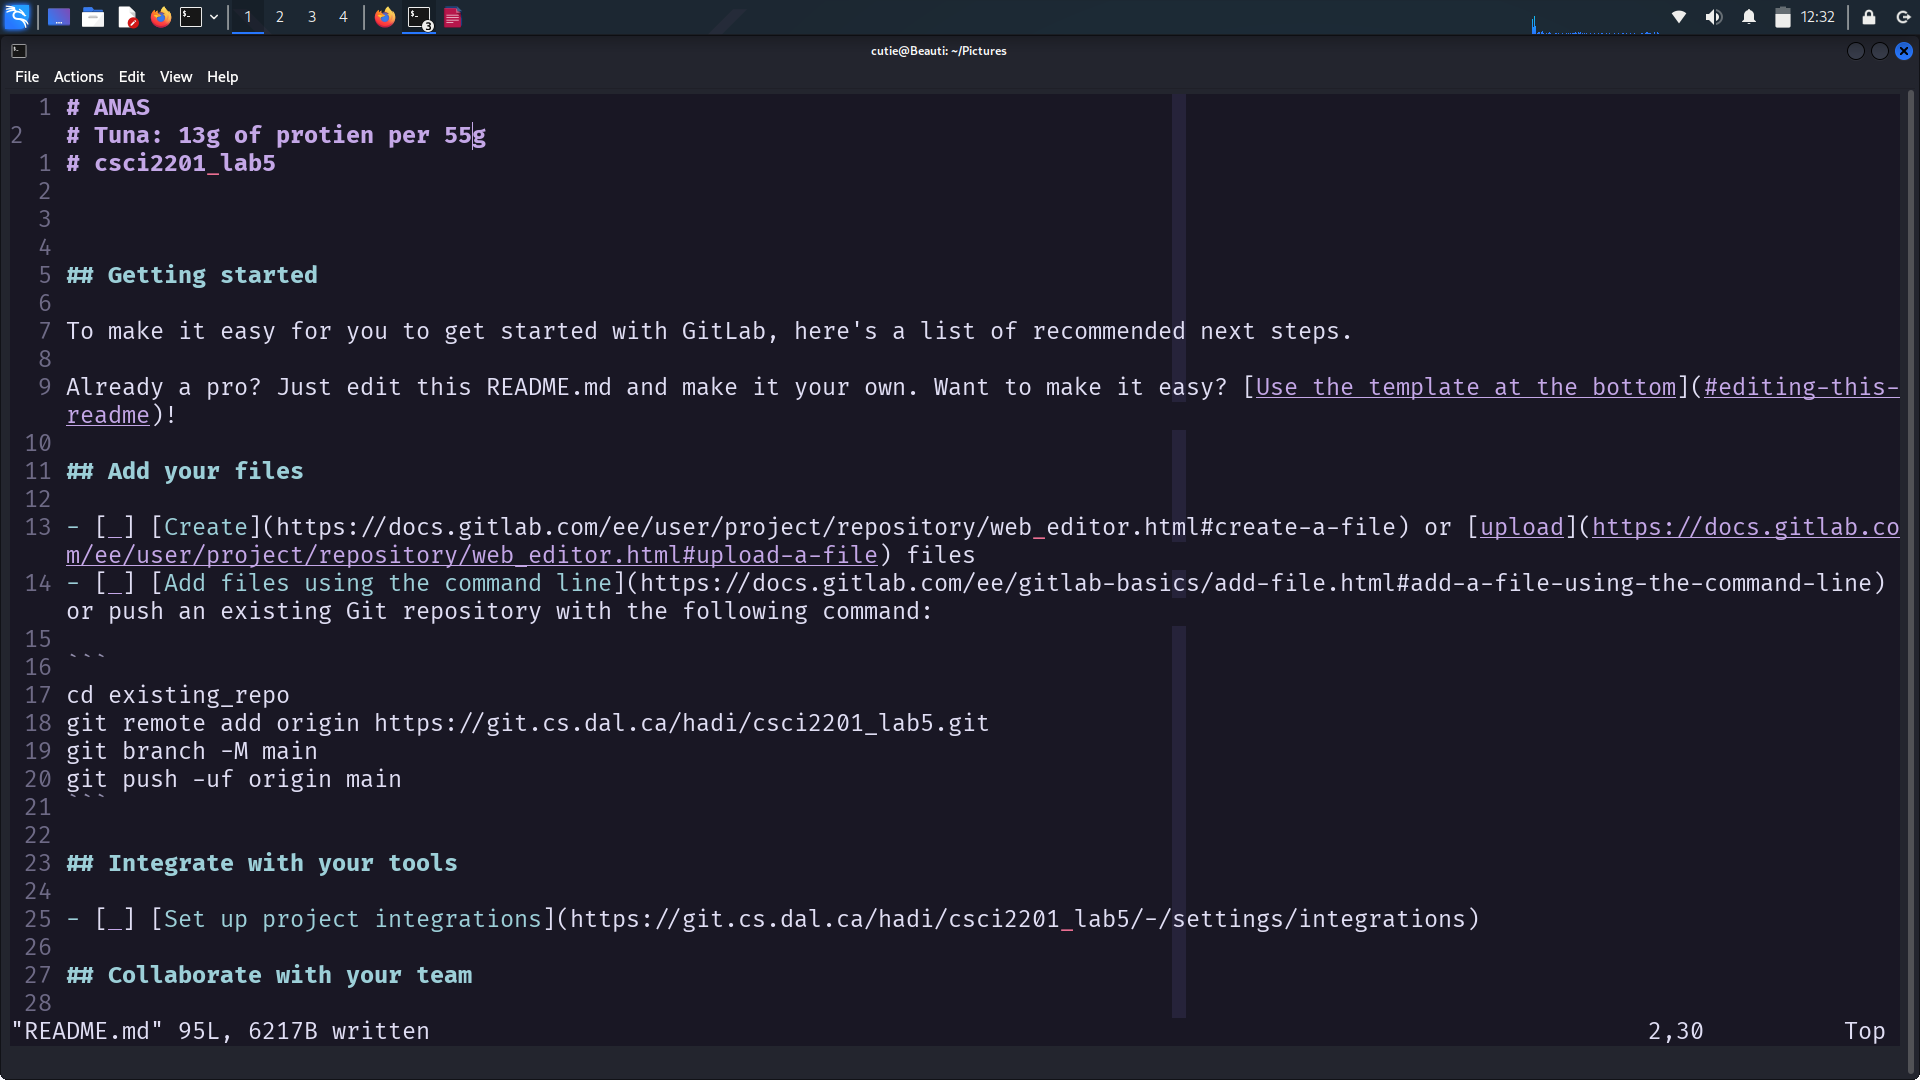
\includegraphics[width=430pt]{pics/Screenshot_2025-03-07_12_32_18.png}
	\end{figure}
	\begin{figure}[H]
		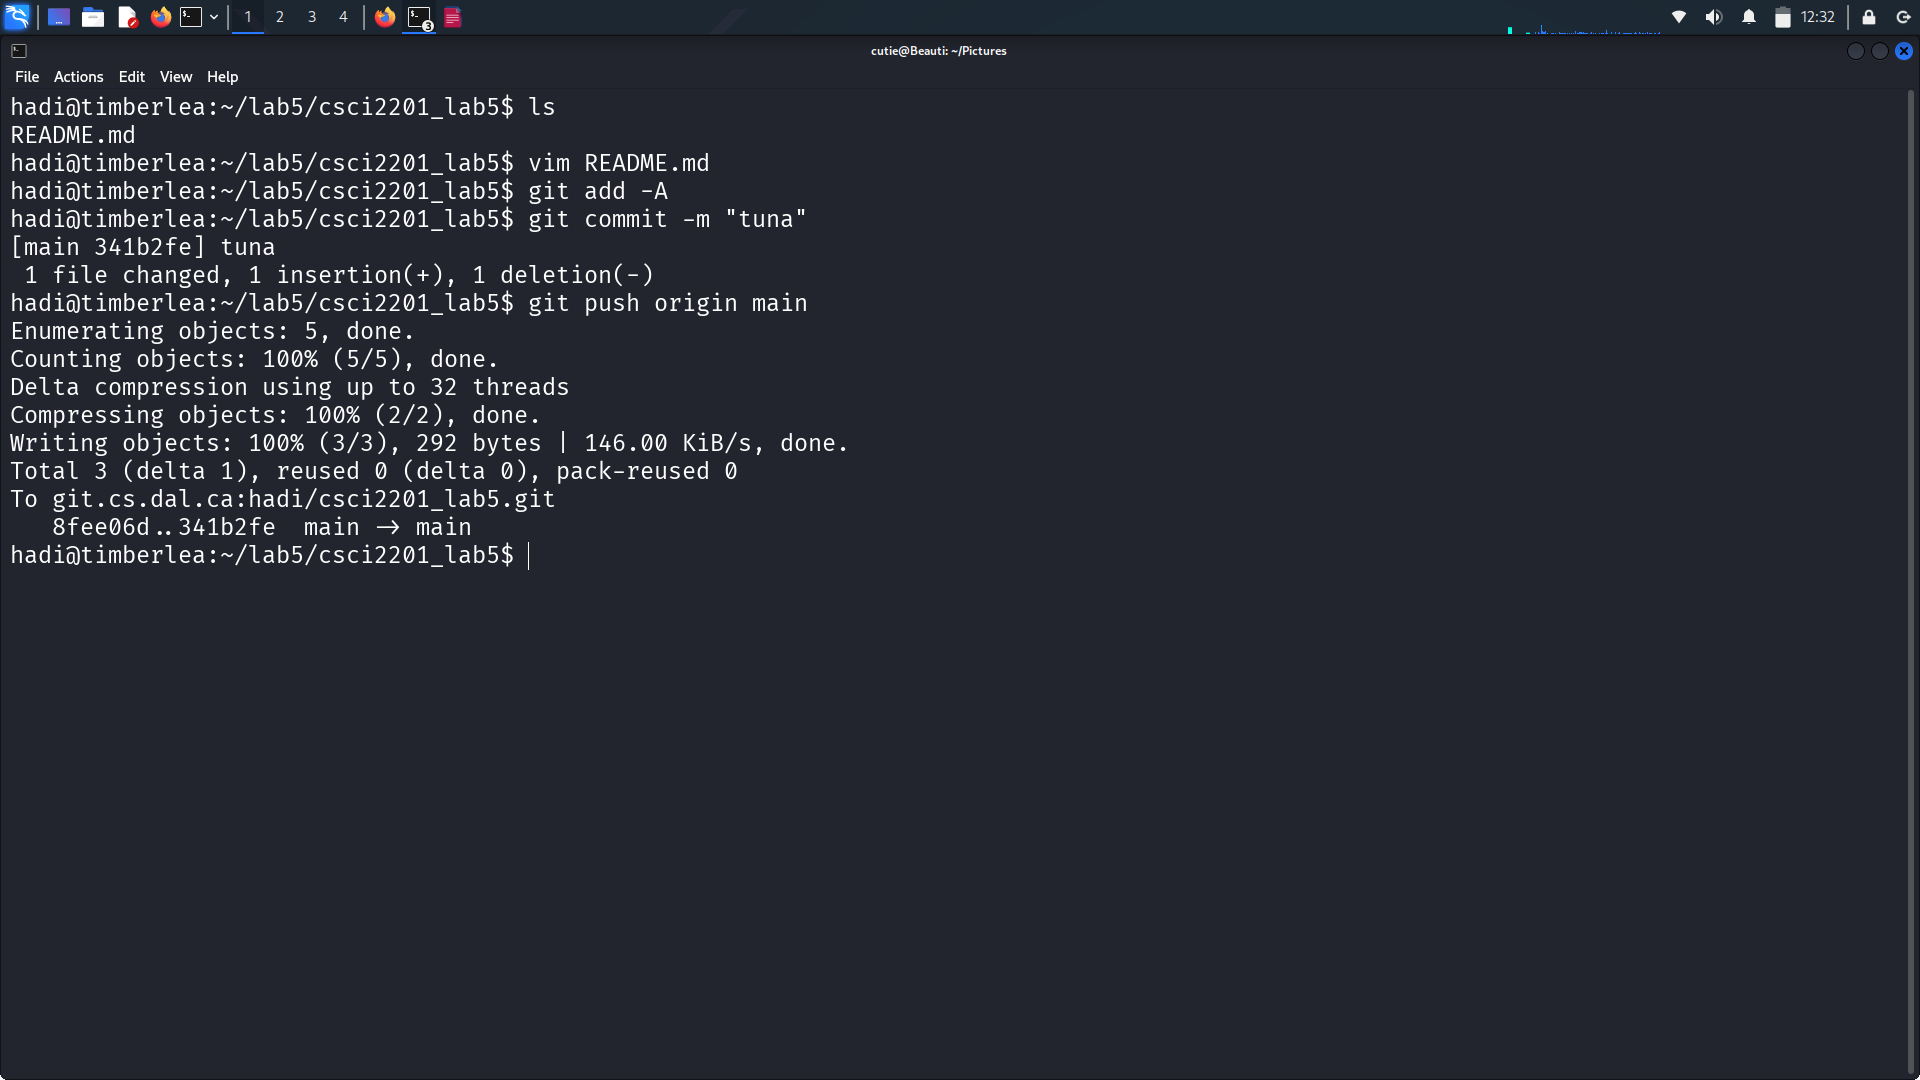
\includegraphics[width=430pt]{pics/Screenshot_2025-03-07_12_32_48.png}
	\end{figure}






	\end{document}
